\documentclass{article}

\IfFileExists{neurips_2024.sty}{
  \usepackage[preprint]{neurips_2024}
}{
  \usepackage[margin=1in]{geometry}
}

\usepackage[utf8]{inputenc}
\usepackage[T1]{fontenc}
\usepackage{microtype}
\usepackage{amsmath}
\usepackage{amssymb}
\usepackage{booktabs}
\usepackage{enumitem}
\usepackage{array}
\usepackage{hyperref}
\usepackage{xcolor}
\usepackage{tikz}
\usetikzlibrary{arrows.meta,positioning}
\IfFileExists{natbib.sty}{\usepackage{natbib}}{}
\providecommand{\citep}[1]{\cite{#1}}

\title{Axon: A Tensors-First Functional Programming Language for Machine Learning Models}

\author{Brainsurgery contributors}

\newcommand{\axon}{\textsc{Axon}}
\newcommand{\graphir}{\textsc{Graph IR}}
\newcommand{\stage}[1]{\textsc{#1}}
\newcommand{\code}[1]{\texttt{#1}}

\begin{document}

\maketitle

\begin{abstract}
Axon is a domain-specific language and compiler pipeline for describing neural
network architectures in a form that remains inspectable, typed, and close to
the parameter structure of modern checkpoints.  The current implementation is
organized as a sequence of explicit source-to-source and source-to-graph
stages.  Each stage consumes a single canonical Axon abstract syntax tree or a
typed graph representation, strengthens a local invariant, and exposes those
invariants to validation and round-trip tests.  This document describes the
system in the style of a conference systems paper: we state the design goals,
define each pipeline contract, and identify the boundary between frontend
normalization, typed core construction, graph lowering, and backend execution.
\end{abstract}

\section{Introduction}

Large language model implementations are usually distributed as a mixture of
Python modules, checkpoint-specific configuration conventions, and tensor
state dictionaries.  This ecosystem is flexible, but it makes independent
analysis, transformation, and backend generation difficult.  A compiler that
targets model families rather than one hand-written implementation per
checkpoint must preserve several kinds of information simultaneously: lexical
names, symbolic dimensions, parameter paths, optional configuration defaults,
control-flow structure, and precise tensor types.

Axon addresses this problem with a small model-description language and a
compiler pipeline that deliberately avoids string-serialization round trips in
semantic stages.  The central design choice is that the pre-lowering compiler
uses one canonical Axon AST.  Stages do not switch to unrelated syntax trees;
instead, they progressively remove surface syntax, resolve names, elaborate
implicit structure, flatten control, and attach inferred metadata.  Graph
lowering then translates the fully typed flat program into an in-memory Graph
IR consumed by code generation and runtime backends.

The goal of this document is not to specify all user-facing Axon syntax.  It is
to make the current pipeline legible as a compiler system: what each stage
accepts, what it guarantees, what it refuses to do, and why those boundaries
matter for correctness and backend portability.

\paragraph{Contributions.}
This document makes three system contributions.  First, it gives a stage
contract for the active Axon compiler path, from source text to typed Graph IR.
Second, it describes how typed metadata and symbolic shape information flow
through the compiler without relying on rendered strings as semantic data.
Third, it defines the backend boundary used by torch, pipeline, runtime, and
tinygrad execution targets.

\section{Design Goals}

\paragraph{Single semantic AST.}
All pre-lowering stages operate on the same Axon AST representation.  A parsed,
resolved, normalized, flattened, and typed program differs by invariants and
metadata, not by changing the meaning of nodes through ad hoc intermediate
formats.

\paragraph{Stage-local contracts.}
Each stage owns a narrow contract.  For example, name resolution does not infer
tensor types; flattening does not repair type errors; backends do not interpret
surface Axon scope syntax.  This separation allows validators and round-trip
tests to target individual compiler properties.

\paragraph{No model-family special casing in the compiler core.}
Model-specific quirks belong in loading and integration paths, not in parsing,
type checking, lowering, graph IR, code generation, runtime, or builtins.
Compiler stages must implement generic language semantics.

\paragraph{Typed graph execution.}
Backends consume a structured, typed Graph IR rather than YAML-like dictionaries
or string-rendered call forms.  This preserves shape and type information for
future backend optimizations and reduces accidental semantic drift.

\section{The Axon Language}

Axon is designed as a compact functional language for model-family
descriptions.  Its first-class domain objects are tensors, symbolic dimensions,
paths into a checkpoint state dictionary, configuration values, and reusable
library definitions.  The language is intentionally biased toward describing
the mathematical structure of a neural network rather than the mechanics of a
specific Python implementation.

\paragraph{Tensors and dimensions first.}
Tensor types carry symbolic shapes.  A type such as
\[
  \code{Tensor[B,S,D]}
\]
states that a value is a tensor whose batch, sequence, and hidden dimensions
are represented by the dimension symbols \(\code{B}\), \(\code{S}\), and
\(\code{D}\).  Dimension symbols are not comments: they participate in
typechecking, unification, primitive type rules, and Graph IR metadata.  This
lets a reusable definition express shape relationships without hard-coding
checkpoint sizes.

\paragraph{Haskell-inspired syntax.}
Definitions use signatures, curried-looking arrows, optional parameters, and a
\code{do}-style statement form:
\begin{verbatim}
block :: Tensor[B,S,D] -> ?Tensor[B,K] -> Tensor[B,S,D]
block x attn_mask = do
  h <- NN.rmsnorm@ln x
  a <- Attention.attention h h h attn_mask
  return x + a
\end{verbatim}
The syntax is not Haskell, but it borrows the idea that signatures are central
documentation and that sequencing should expose dataflow explicitly.  Pipes
and scoped parameter paths are surface conveniences that are normalized away
before flattening.

\paragraph{Functional semantics.}
Axon definitions are pure functions over explicit arguments, configuration
lookups, and parameter-path reads.  A bind statement names the value produced
by an expression.  Except for ternary branch expressions, expressions are
eager: a call used as an argument is evaluated before the callee receives the
value.  This eagerness is important for flattening and for preserving the
semantics of computations with expensive tensor operations.

\paragraph{Paths and reusable libraries.}
Checkpoint parameters are accessed through typed path values.  Relative path
sugar is lexical authoring syntax; the flat core uses ordinary \code{Path}
arguments and absolute or templated absolute paths.  Reusable library modules
such as \code{NN}, \code{Tensor}, \code{Attention}, \code{Masking}, \code{MoE},
\code{Cache}, and \code{Positions} define model-independent operations.  Model
files combine these libraries with checkpoint-specific configuration paths and
architecture-level control.

\paragraph{Semantic core.}
The compiler treats the surface language as notation for a smaller core.  The
core contains explicit calls, explicit path arguments, flat bindings, helper
definitions for loops, and typed primitive calls.  Optional and default
parameters are represented through ordinary call arguments and keyword
arguments according to the elaboration contract, rather than through backend
fallbacks.  Backend implementations consume Graph IR derived from this core;
they do not implement surface Axon syntax.

\section{Type System, Checking, and Inference}

The active type system is implemented by \code{typecheck2}.  It is not a
separate backend contract and it is not the removed legacy checker.  Its input
is a flat, closed Axon AST after normalization, elaboration, and flattening;
its output is the same AST with typed module signatures and per-expression
metadata.  The checker is MAIN-module based: it resolves the effective MAIN
module, computes the reachable definition graph, prunes unreachable
definitions, checks demanded definitions from MAIN, and validates the typed
result.

\paragraph{Types.}
The implemented type language includes \code{Any}, \code{Bool}, \code{Dim},
\code{Float}, \code{Int}, \code{Null}, \code{Path}, \code{String},
\code{List[T]}, tuples, optionals \code{?T}, tensor types
\[
  \code{Tensor}[d_1,\ldots,d_n],
\]
tensor sub-bases such as \code{IdxTensor[...]}, named type aliases, and
generated type variables.  Dimension tokens may be integer literals, symbolic
names, variadic binders such as \code{..S}, or symbolic expressions over
\(+\), \(-\), \(*\), and \(/\).  Type aliases are expanded during unification
and normalization, including aliases with variadic dimension parameters.

\paragraph{Expression metadata.}
The typing judgment can be read operationally as
\[
  \Gamma \vdash e \Rightarrow (e^\tau,\tau,a,d),
\]
where \(\Gamma\) contains term bindings, desugared \code{Path} bindings,
dimension-name bindings, module definitions, aliases, expression aliases,
type-variable substitutions, and dimension substitutions.  The result is a
typed expression \(e^\tau\), inferred type \(\tau\), inferred arity \(a\), and
inferred tensor dimensions \(d\) when applicable.  Typed validation rejects
missing arity metadata and rejects tensor expressions without inferred
dimensions.

\paragraph{Literals, ascriptions, and numeric inference.}
Variables are typed by environment lookup.  Unbound names are type errors.
Literals initially receive their natural scalar types: integers are
\code{Int}, floats are \code{Float}, booleans are \code{Bool}, strings are
\code{String}, \code{null} is \code{Null}, and path literals are \code{Path}.
Type ascriptions \((e :: T)\) are checked rather than erased: the inferred
type of \(e\) is unified with \(T\), and the ascription remains in the typed
AST.  Numeric unification is deliberately pragmatic: \code{Int} with
\code{Float} yields \code{Float}, \code{Dim} with \code{Float} yields
\code{Float}, and \code{Int} with \code{Dim} yields \code{Dim}.  Numeric
literals are retagged in typed contexts, e.g. integer literals inside
\code{List[Dim]} shape arguments become dimension literals.

\paragraph{Unification and dimension names.}
Unification first applies substitutions and expands aliases.  Type variables
bind with an occurs check; \code{Any} unifies with and yields the other side;
lists, tuples, optionals, named types, and tensor types unify structurally.
Tensor unification checks compatible bases and dimension sequences.  The
generic base \code{Tensor} can unify with more specific tensor bases, while
incompatible non-generic bases are rejected.  Dimension unification supports
ordinary symbols, integer literals, variadic dimension binders, and symbolic
binary expressions.  It simplifies common arithmetic identities, rejects
recursive dimension bindings, and prefers readable existing names over
generated names when two dimensions are equivalent.

\paragraph{Calls and call-site specialization.}
User definitions, builtin Axon definitions, and generated helpers all use the
same call path.  At a call site, the callee signature is instantiated with
fresh type and dimension variables, explicit path arguments are consumed first,
actual arguments are typed, and actual types are unified with formal parameter
types.  Dimension-typed actual expressions are also used to bind fresh
signature dimensions to source-level dimension names.  When safe, typecheck2
checks the callee body under the call-site environment and uses the specialized
body return type if it is more precise than the declared header.  Caller
substitutions are restored afterward so local inference does not leak
arbitrarily across calls.  Recursive calls use the current instantiated
interface when the callee is already active.

\paragraph{Primitive rules.}
Primitive calls are registered in \code{brainsurgery/synapse/ops}.  Each
primitive provides \code{OP\_NAME} and a \code{LOWERING\_TYPE\_SIGNATURE}; it
may additionally provide a \code{type\_rule} hook.  Typecheck2 checks actuals
against the lowering signature, rejects explicit \code{null} where a
non-optional primitive parameter is required, then lets the primitive rule
compute a more precise result type when necessary.  This is where rules for
shape-transforming operations such as \code{reshape}, \code{expand},
\code{permute}, \code{transpose}, \code{chunk}, \code{split}, \code{concat},
and \code{slice} live, as well as neural-network primitives such as
\code{embedding}, \code{linear}, \verb|expert_linear|, \code{layernorm}, and
\code{rmsnorm}.

\paragraph{Branches, nullability, and returns.}
Ternaries and expression-level \code{if} require boolean conditions.  Branch
types are joined structurally: tuples itemwise, optionals by joining inner
types, and tensors by preserving equivalent dimensions or using broadcasting
where appropriate.  Null checks refine environments: in a branch guarded by
\code{x == null} or \code{x != null}, a value of type \code{?T} is treated as
\code{Null} on the null side and \(T\) on the non-null side.  Return and yield
statements are checked against declared return types when available, while
preserving protected header dimension names so literals or generated call-site
names do not overwrite meaningful signature dimensions.

\paragraph{Destructuring and generated helpers.}
Multi-target binds destructure tuples of matching arity, lists by repeating
the list item type, and unconstrained type variables by binding them to tuples
of fresh type variables.  Generated loop and branch helpers are ordinary
definitions: they do not have a compatibility typing mode.  After checking,
generated helper signatures and body annotations are normalized and
canonicalized.  Typecheck2 repeats the pass up to a fixed bound and returns
once the typed AST reaches a deterministic fixpoint; short equivalent-name
cycles are broken by choosing a deterministic structural spelling.

\paragraph{Current limits.}
The active checker does not expose a complete public constraint store over
dimensions, integers, booleans, and nullability.  Some broad primitive
signatures still rely on primitive-specific hooks for precision.  Unknown
keyword arguments on user calls are still permissively carried by the checker,
although later validation or lowering may reject them.  These are
implementation facts, not intended backend escape hatches.

\section{System Model}

An Axon compilation unit consists of model-family source files, builtin Axon
definitions, checkpoint metadata, and a selected main definition.  The compiler
must support both generic model-family files and materialized checkpoint
variants.  A model definition may reference symbolic dimensions, configuration
values, optional cache values, parameter paths, scoped parameter templates, and
builtin neural-network operations.

The compiler has two semantic representation families.  The first is the Axon
AST used by all frontend and typed-core stages.  The second is Graph IR, a
typed SSA-like representation inspired by standard compiler dataflow
representations such as SSA~\citep{cytron1991ssa}.  Flattening uses an
administrative-normal-form style decomposition of nested expressions into
explicit binds, similar in spirit to ANF/CPS compiler normal forms
\citep{sabry1992anf}.  Backend execution currently targets PyTorch
\citep{paszke2019pytorch} and tinygrad.

\section{Compiler Invariants}

The most important invariant is monotonicity of structure: later stages should
see fewer surface constructs and more metadata, never weaker semantic
information.  For example, after resolution, there should be no unresolved
imports; after normalization, there should be no callee path sugar; after
flattening, there should be no statement-level control; after typecheck2, graph
lowering should not need to infer missing tensor types.

The second invariant is backend isolation.  Backend implementations may choose
different tensor libraries and primitive implementations, but they must consume
the same Graph IR contract.  If a backend requires weaker validation or
model-family-specific dispatch to run, the issue belongs either in the backend
implementation or in an explicitly approved language extension.

\section{Pipeline Overview}

The current default path is shown below.  Optional optimization is separated
from the correctness-critical path; the backend path is expected to work
without the AST optimizer.

\begin{figure}[t]
\centering
\fbox{\begin{minipage}{0.92\linewidth}
\centering
source Axon
\(\rightarrow\) parse/load/materialize
\(\rightarrow\) resolve/validate
\(\rightarrow\) normalize/elaborate
\(\rightarrow\) flatten
\(\rightarrow\) typecheck2
\(\rightarrow\) Graph IR
\(\rightarrow\) backend execution
\end{minipage}}
\caption{Default Axon compilation path.  Optional optimization is excluded from
the correctness-critical path in this paper.}
\label{fig:pipeline}
\end{figure}

\begin{figure}[t]
\centering
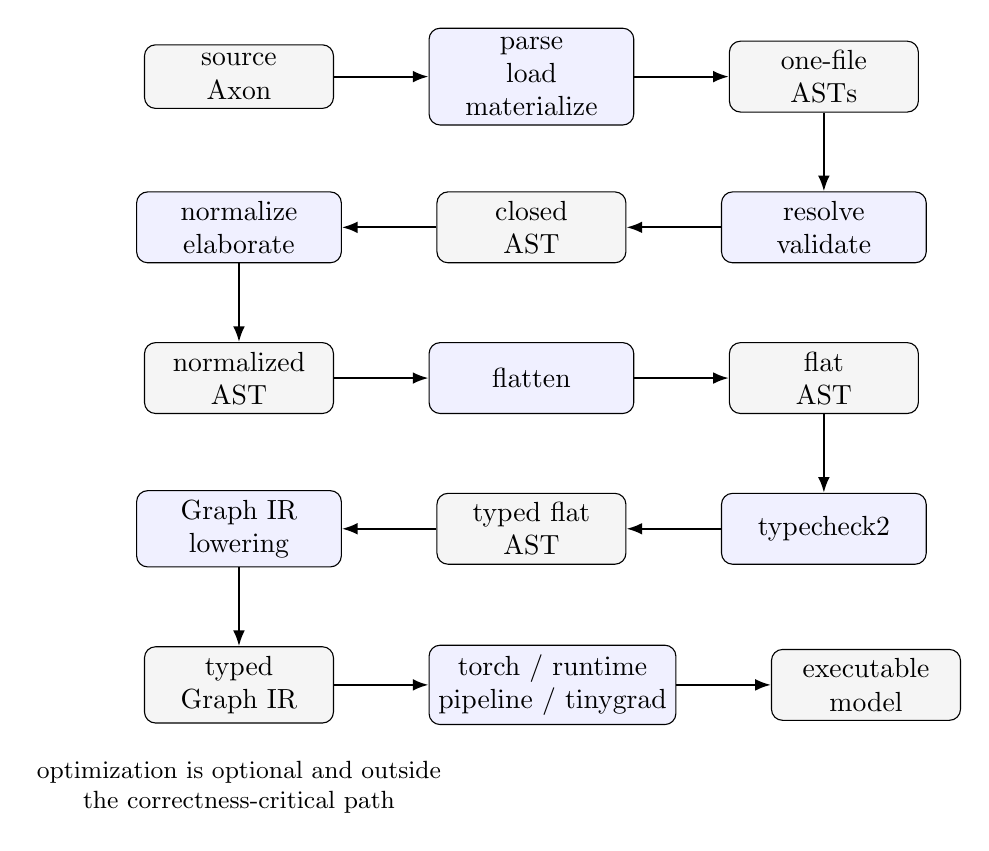
\begin{tikzpicture}[
  stagebox/.style={draw, rounded corners, fill=blue!6, align=center, minimum width=2.6cm, minimum height=0.9cm},
  repbox/.style={draw, rounded corners, fill=gray!8, align=center, minimum width=2.4cm, minimum height=0.7cm},
  edge/.style={-{Latex[length=2mm]}, thick},
  note/.style={align=center, font=\small}
]
\node[repbox] (src) {source\\Axon};
\node[stagebox, right=1.2cm of src] (parse) {parse\\load\\materialize};
\node[repbox, right=1.2cm of parse] (onefile) {one-file\\ASTs};
\node[stagebox, below=1.0cm of onefile] (resolve) {resolve\\validate};
\node[repbox, left=1.2cm of resolve] (closed) {closed\\AST};
\node[stagebox, left=1.2cm of closed] (norm) {normalize\\elaborate};
\node[repbox, below=1.0cm of norm] (normast) {normalized\\AST};
\node[stagebox, right=1.2cm of normast] (flatten) {flatten};
\node[repbox, right=1.2cm of flatten] (flat) {flat\\AST};
\node[stagebox, below=1.0cm of flat] (tc) {typecheck2};
\node[repbox, left=1.2cm of tc] (typed) {typed flat\\AST};
\node[stagebox, left=1.2cm of typed] (lower) {Graph IR\\lowering};
\node[repbox, below=1.0cm of lower] (graph) {typed\\Graph IR};
\node[stagebox, right=1.2cm of graph] (backend) {torch / runtime\\pipeline / tinygrad};
\node[repbox, right=1.2cm of backend] (exec) {executable\\model};

\draw[edge] (src) -- (parse);
\draw[edge] (parse) -- (onefile);
\draw[edge] (onefile) -- (resolve);
\draw[edge] (resolve) -- (closed);
\draw[edge] (closed) -- (norm);
\draw[edge] (norm) -- (normast);
\draw[edge] (normast) -- (flatten);
\draw[edge] (flatten) -- (flat);
\draw[edge] (flat) -- (tc);
\draw[edge] (tc) -- (typed);
\draw[edge] (typed) -- (lower);
\draw[edge] (lower) -- (graph);
\draw[edge] (graph) -- (backend);
\draw[edge] (backend) -- (exec);

\node[note, below=0.35cm of graph] {optimization is optional and outside\\the correctness-critical path};
\end{tikzpicture}
\caption{Staged Axon pipeline.  Blue boxes are transformations; gray boxes are
representations with stronger invariants than the previous representation.}
\label{fig:pipeline-tikz}
\end{figure}

\begin{center}
\begin{tabular}{lll}
\toprule
Phase & Representation & Primary invariant \\
\midrule
Parse/load/materialize & one-file ASTs & syntactic structure and checkpoint defaults \\
Resolve/validate & closed AST & no unresolved imports or names \\
Normalize/elaborate & normalized AST & explicit call and default/defaultable structure \\
Flatten & flat AST & no statement-level control or relative paths \\
Typecheck2 & typed flat AST & expression types, arities, and dimensions \\
Graph lowering & Graph IR & typed SSA-like graph modules \\
Backend & generated/runtime code & executable tensor program \\
\bottomrule
\end{tabular}
\end{center}

The following sections describe the stages in order.

\section{Running Example}

This section follows a small Axon fragment through the main representations.
The example is intentionally smaller than a full transformer block, but it
uses the same mechanisms: path sugar, a defaulted keyword argument, tensor
shapes, nested calls, and typed graph lowering.

\paragraph{Surface Axon.}
A model author can write a reusable projection with a concise functional form:
\begin{verbatim}
project :: Tensor[B,S,D] -> Tensor[B,S,O]
project x = do
  y <- Tensor.reshape x shape=[B, S, D]
       |> NN.linear@proj dim=O
  return y
\end{verbatim}
The surface program contains a pipe, callee-attached path sugar
\code{@proj}, a shape expression, and an omitted default argument such as
\code{bias=true} from the library definition of \code{NN.linear}.

\paragraph{Normalize and elaborate.}
Normalization removes pipe syntax and path sugar by turning them into ordinary
call structure.  Elaboration then accounts for defaultable parameters declared
by the callee signature:
\begin{verbatim}
project x = do
  y <- NN.linear @proj
         (Tensor.reshape x shape=[B, S, D])
         dim=O bias=true
  return y
\end{verbatim}
The point is not that all defaults must always be textually present in user
source.  The invariant is that downstream stages see a call surface whose
provided positional, keyword, and path arguments are unambiguous.

\paragraph{Flatten.}
Flatten preserves eager evaluation order by introducing explicit binds and by
making paths absolute or templated absolute values:
\begin{verbatim}
project :: Tensor[B,S,D] -> Tensor[B,S,O]
project x = do
  _v1 <- Tensor.reshape x shape=[B, S, D]
  y <- NN.linear @@proj _v1 dim=O bias=true
  return y
\end{verbatim}
The flat program has no pipe expression, no nested call used as an argument,
and no callee path sugar.  It is still Axon source, but it is now in the core
form expected by typecheck2 and Graph IR lowering.

\paragraph{Typecheck2.}
Typecheck2 annotates every expression with type, arity, and tensor-dimension
metadata.  The same flat program can be read as:
\begin{verbatim}
_v1 <- (Tensor.reshape (x :: Tensor[B,S,D])
          shape=([B, S, D] :: List[Dim]) :: Tensor[B,S,D])
y <- (NN.linear (@@proj :: Path) (_v1 :: Tensor[B,S,D])
        dim=(O :: Dim) bias=(true :: Bool) :: Tensor[B,S,O])
\end{verbatim}
The important information is not the exact rendered punctuation, but the fact
that the tensor shape relation \(x : \code{Tensor[B,S,D]}\) and
\(y : \code{Tensor[B,S,O]}\) is explicit before lowering.

\paragraph{Graph IR.}
Lowering turns each flat bind into a typed graph node.  A schematic graph
module is:
\begin{verbatim}
module project(x: Tensor[B,S,D]) -> Tensor[B,S,O]
  n1 = call Tensor.reshape(
         x, shape=[B,S,D]) -> Tensor[B,S,D]
  n2 = call NN.linear(
         path=@@proj, x=n1, dim=O, bias=true)
       -> Tensor[B,S,O]
  return n2
\end{verbatim}
Backends receive this structured graph object, not a string-rendered Axon
program.  Torch, pipeline, runtime, and tinygrad implementations therefore
share the same typed operands, path values, and output types.

\begin{figure}[t]
\centering
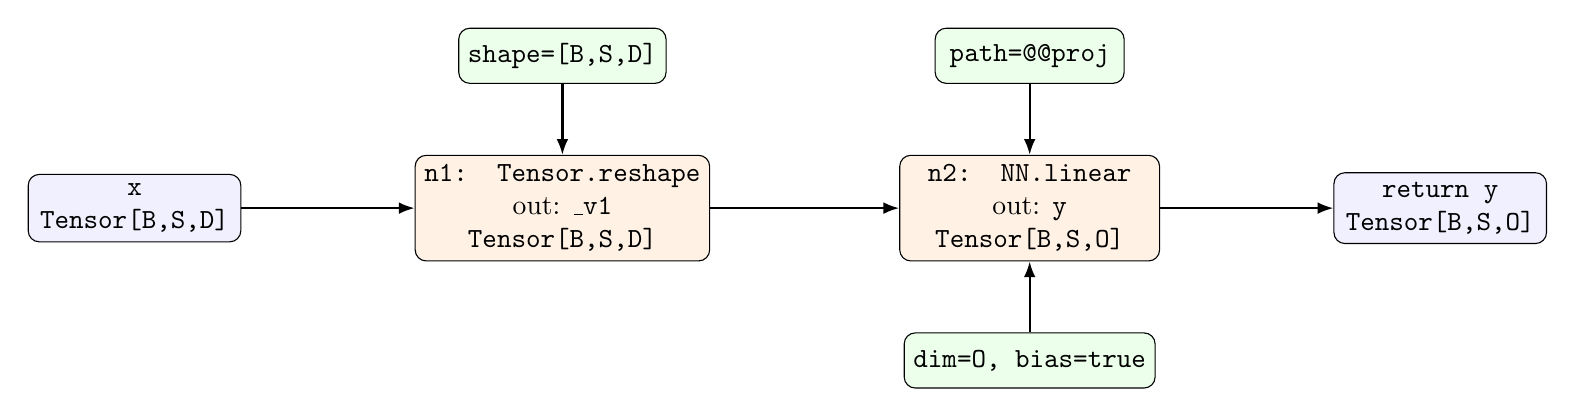
\begin{tikzpicture}[
  value/.style={draw, rounded corners, fill=blue!6, align=center, minimum width=2.7cm, minimum height=0.8cm},
  nodeop/.style={draw, rounded corners, fill=orange!10, align=center, minimum width=3.3cm, minimum height=1.0cm},
  attr/.style={draw, rounded corners, fill=green!8, align=center, minimum width=2.4cm, minimum height=0.7cm},
  edge/.style={-{Latex[length=2mm]}, thick}
]
\node[value] (x) {\code{x}\\\code{Tensor[B,S,D]}};
\node[nodeop, right=2.2cm of x] (reshape) {\code{n1: Tensor.reshape}\\out: \code{\_v1}\\\code{Tensor[B,S,D]}};
\node[nodeop, right=2.4cm of reshape] (linear) {\code{n2: NN.linear}\\out: \code{y}\\\code{Tensor[B,S,O]}};
\node[value, right=2.2cm of linear] (ret) {\code{return y}\\\code{Tensor[B,S,O]}};

\node[attr, above=0.9cm of reshape] (shape) {\code{shape=[B,S,D]}};
\node[attr, above=0.9cm of linear] (path) {\code{path=@@proj}};
\node[attr, below=0.9cm of linear] (attrs) {\code{dim=O, bias=true}};

\draw[edge] (x) -- (reshape);
\draw[edge] (reshape) -- (linear);
\draw[edge] (linear) -- (ret);
\draw[edge] (shape) -- (reshape);
\draw[edge] (path) -- (linear);
\draw[edge] (attrs) -- (linear);
\end{tikzpicture}
\caption{Graph IR view of the running example.  Rectangles denote typed graph
values and operation nodes.  Paths, literals, and shape lists are structured
operands or attributes, not strings that backends must parse.}
\label{fig:running-graph-ir}
\end{figure}

\paragraph{Why the stages matter.}
The example illustrates the intended division of labor.  Normalize removes
surface notation; elaborate resolves the defaultable call surface; flatten
exposes evaluation order; typecheck2 attaches shape and arity metadata; Graph
IR lowering produces backend-neutral typed dataflow.  No backend has to know
how \code{|>}, \code{@proj}, lexical scopes, or omitted defaults were written
in the source program.

\section{Parse}

\paragraph{Input and output.}
The parse stage consumes Axon source text and produces a one-file Axon AST.
It records syntactic structure, source-level names, declarations, imports,
exports, pragmas, type ascriptions, path literals, and expression forms.

\paragraph{Contract.}
Parsing is intentionally syntax-local.  It does not load imported files,
resolve names, infer types, normalize call syntax, materialize configuration
values, or lower operations.  A parse result may contain unresolved references
and surface sugar; those are obligations of later stages.

\paragraph{Rationale.}
Keeping parse pure makes it possible to test grammar stability independently
from the file system and from checkpoint availability.  It also prevents the
parser from becoming an implicit compatibility layer for downstream stages.

\paragraph{Formal view.}
Let \(\Sigma\) be source text and \(A_f\) be a one-file Axon AST.  Parse is a
partial function
\[
  \mathsf{parse}: \Sigma \rightharpoonup A_f .
\]
It is undefined for syntactically invalid programs, but it is defined for
programs with unresolved identifiers, unresolved imports, or type errors.

\paragraph{Example.}
The source fragment
\begin{verbatim}
import NN

embed :: Tensor[B,S] -> Tensor[B,S,D]
embed ids = NN.embedding@wte ids dim=D
\end{verbatim}
is parsed into an import declaration, a typed definition, a parameter list, and
a call expression whose callee still carries surface path sugar
\code{@wte}.  Parse records this structure but does not decide whether
\code{NN.embedding} exists or whether \code{D} is a valid dimension symbol.

\section{Load}

\paragraph{Input and output.}
The load stage consumes a root one-file AST plus origin-path information and
returns the root program together with the imported Axon files needed by that
program.

\paragraph{Contract.}
Loading is responsible for file discovery and import-root policy.  It does not
merge modules, rewrite references, prune unreachable definitions, or infer
types.  The output is still a collection of one-file ASTs.

\paragraph{Rationale.}
Separating loading from parsing keeps source-text parsing deterministic and
lets resolution operate over an explicit import set.  This also makes it easier
to test imported builtins and model files without hiding file-system effects in
the parser.

\paragraph{Formal view.}
For a root AST \(A_0\), an origin path \(p\), and an import search policy
\(\mathcal{I}\), loading computes a finite import closure:
\[
  \mathsf{load}(A_0,p,\mathcal{I}) = [A_0,A_1,\ldots,A_n].
\]
The result is ordered only for deterministic processing; it is not yet a
single linked program.

\paragraph{Example.}
If a model file imports
\begin{verbatim}
import NN
import Attention (attention, reshape_heads)
\end{verbatim}
load finds the corresponding builtin Axon files and parses them.  The model AST
still contains import declarations, and the imported ASTs remain separate
files.  Qualified names such as \code{Attention.attention} are not resolved
until the next stage.

\section{Materialize}

\paragraph{Input and output.}
Materialization consumes a generic one-file Axon AST and checkpoint metadata.
It emits a one-file Axon AST specialized enough to be inspected or used as a
checkpoint-specific artifact.

\paragraph{Contract.}
The stage may resolve materialization-specific configuration expressions, but
it must not become an optimizer.  It does not perform dead-code elimination,
general constant folding, alias expansion, inlining, type inference, or
backend-specific rewriting.

\paragraph{Rationale.}
Generic model files are the source of truth for model families.  Materialized
files are useful for inspection and targeted debugging, but materialization
must not silently repair or reinterpret the program in ways that diverge from
the generic source.

\paragraph{Formal view.}
For generic AST \(A_f\) and checkpoint metadata \(C\), materialization is a
source-to-source transformation
\[
  \mathsf{materialize}(A_f,C) = A_f'
\]
that may replace materialization-approved configuration expressions with
checkpoint-specific values.  It must preserve the program's definition graph
and must not depend on backend selection.

\paragraph{Example.}
A generic constant may be written as
\begin{verbatim}
MODEL_DIM = Config.int@@hidden_size default=768
\end{verbatim}
For a checkpoint whose configuration contains \verb|hidden_size = 1024|,
materialization may emit
\begin{verbatim}
MODEL_DIM = 1024
\end{verbatim}
It should not also inline all uses of \verb|MODEL_DIM|, delete unused branches,
or specialize unrelated functions.

\section{Resolve}

\paragraph{Input and output.}
Resolution consumes the loaded set of one-file ASTs and produces a single
closed Axon AST.

\paragraph{Contract.}
Resolve merges imported modules, resolves qualified and unqualified references,
checks export visibility, removes import-surface state, identifies the main
module, and prunes definitions that are unreachable from the main module under
the current compilation mode.

\paragraph{Exclusions.}
Resolve does not typecheck expressions, infer dimensions, lower operations, or
apply warning policy.  Diagnostics such as unused imports or strict warning
promotion belong to validation or orchestration.

\paragraph{Rationale.}
Downstream stages should never need to search the file system or infer lexical
scope from import declarations.  They receive one closed program with explicit
definition identities.

\paragraph{Formal view.}
Resolution maps a finite set of one-file ASTs to one closed AST:
\[
  \mathsf{resolve}: [A_f] \rightharpoonup A_c .
\]
The function is undefined when imports are missing, exported names are
ambiguous, or reachable expressions reference undefined names.  The output
\(A_c\) has no import-surface state in the reachable program.

\paragraph{Example.}
Given
\begin{verbatim}
import Tensor (reshape)

f x = reshape x shape=[B, S, D]
\end{verbatim}
resolve links \code{reshape} to the imported \code{Tensor.reshape}
definition.  If both \code{Tensor.reshape} and another imported \code{reshape}
are available unqualified, resolution reports ambiguity rather than choosing
one.

\section{Validate}

\paragraph{Input and output.}
Validation consumes a closed AST and returns the same AST when the requested
invariant set holds.  On failure, it reports diagnostics rather than producing
a repaired program.

\paragraph{Contract.}
The pre-flatten validator checks closedness, unresolved-name rejection,
type-alias arity and visibility, and structural properties required before
normalization and flattening.  Later validators check stronger stage-specific
properties such as normalized calls, flat control, backend-required graph shape,
and typed metadata consistency.

\paragraph{Rationale.}
Validation is a certification layer, not a transformation layer.  This is what
lets later stages reject invalid inputs instead of weakening their assumptions.

\paragraph{Formal view.}
A validator is a predicate over an AST representation:
\[
  \mathsf{validate}_k(A) =
  \begin{cases}
  A & \text{if invariant set } k \text{ holds},\\
  \bot & \text{otherwise.}
  \end{cases}
\]
The returned AST is structurally identical to the input.  Diagnostics are
separate from transformation.

\paragraph{Example.}
Before flattening, validation rejects a closed program that still contains a
reachable unresolved name:
\begin{verbatim}
f x = does_not_exist x
\end{verbatim}
After flattening, a stronger validator rejects statement-level control:
\begin{verbatim}
if cond then do
  y <- f x
else do
  y <- g x
\end{verbatim}
because flat Axon must express this through values, helpers, or ternaries.

\section{Normalize}

\paragraph{Input and output.}
Normalize consumes a validated closed AST and emits a normalized closed AST.

\paragraph{Contract.}
The stage removes call and control sugar that would otherwise complicate
flattening.  Callee path suffixes become ordinary \code{Path}-typed arguments,
pipe syntax becomes ordinary calls, callable-name expressions that denote
zero-argument calls become explicit calls, and loop bodies receive explicit
yield/carry protocol structure.

\paragraph{Exclusions.}
Normalize does not globally expand default arguments.  Defaults are handled by
the elaboration stage and by type-aware binding where appropriate.

\paragraph{Rationale.}
Normalize is the boundary between surface authoring syntax and a regularized
AST.  It keeps later stages from duplicating parser-level sugar handling.

\paragraph{Formal view.}
Normalize is a total transformation over validated closed ASTs:
\[
  \mathsf{normalize}: A_c \rightarrow A_n .
\]
It preserves denotation while reducing the number of syntactic forms.  The
validator for \(A_n\) checks that eliminated sugar does not reappear.

\paragraph{Example: path and pipe sugar.}
The surface expression
\begin{verbatim}
x <- input |> NN.layernorm@ln_f eps=1e-5
\end{verbatim}
normalizes to an ordinary call whose path is an explicit argument:
\begin{verbatim}
x <- NN.layernorm @ln_f input eps=1e-5
\end{verbatim}
The exact rendered form may differ, but the AST no longer represents either a
pipe expression or callee-attached path sugar.

\paragraph{Example: loop protocol.}
A source loop with implied carry/yield is normalized so that the loop body has
an explicit final yield.  Flattening therefore sees one loop protocol rather
than several authoring conveniences.

\section{Elaborate}

\paragraph{Input and output.}
Elaboration consumes a normalized closed AST and produces a closed AST with
implicit call structure made explicit where the language contract requires it.

\paragraph{Contract.}
The current elaboration stage is signature-aware and focuses on the boundary
between surface calls and the flat core.  It preserves user-visible type
ascriptions and does not erase inferred metadata.  Its job is to make
defaultable call structure explicit enough that flattening, typecheck2, and
Graph IR lowering do not need ad hoc fallback logic for omitted optional
parameters.

Elaboration accounts for already-supplied positional arguments, explicit
keyword arguments, path arguments introduced by normalization, and optional
parameters with implicit \code{null} defaults.  It adds a missing keyword
argument only when the corresponding formal parameter is not already covered by
the call.  This is part of the round-trip contract: flat rendered Axon
represents scoped calls with ordinary leading \code{Path} arguments, and
reparsing such a program preserves the same call surface instead of adding
duplicate defaults for parameters supplied positionally.

\paragraph{Rationale.}
Elaboration sits after normalization because normalization first determines
which expressions are calls.  Once calls are explicit, elaboration can apply
signature-aware rules without reinterpreting syntax.

\paragraph{Formal view.}
For normalized AST \(A_n\), elaboration produces \(A_e\):
\[
  \mathsf{elaborate}: A_n \rightarrow A_e .
\]
The transformation is signature-aware but not type-inferential.  For a call
\(\code{f}\ a_1 \ldots a_m\ \{k_j=v_j\}\), it binds actual arguments to the
callee surface after accounting for path slots and positional parameters.  For
each remaining formal parameter \(p\), elaboration may insert \(p=d_p\) when
\(p\) has a declared default \(d_p\), or \(p=\code{null}\) when \(p\) is
optional without an explicit default.  It does not solve tensor shapes.

The stage is idempotent under the weak and strong round-trip tests used for
model Axon files: rendering and reparsing an elaborated artifact, with or
without re-running earlier resolution, yields the same elaborated call
structure.

\paragraph{Example.}
If a library function has the signature
\begin{verbatim}
linear :: Path -> Tensor[B,S,D] -> ?Dim -> ?Bool -> Tensor[B,S,O]
linear path x ?dim=null ?bias=true = ...
\end{verbatim}
then a call such as
\begin{verbatim}
y <- NN.linear @w x
\end{verbatim}
can be elaborated to an equivalent call with explicit defaulted arguments:
\begin{verbatim}
y <- NN.linear @w x dim=null bias=true
\end{verbatim}
This prevents downstream stages from inventing backend-specific defaults.
However, if a call already supplies the optional parameter positionally,
elaboration does not also add the keyword form:
\begin{verbatim}
y <- f path x supplied_optional
\end{verbatim}
must remain a single binding of the optional formal, not become
\begin{verbatim}
y <- f path x supplied_optional optional=null
\end{verbatim}
after rendering and reparsing.

\section{Flatten}

\paragraph{Input and output.}
Flatten consumes an elaborated closed AST and emits a flat closed Axon AST.

\paragraph{Contract.}
The flat program has no statement-level \code{if}, no \code{for}, no
\code{scope}, no relative paths, and no hidden callee path sugar.  Complex
expressions are lowered into explicit bind statements, loop constructs are
converted into helper definitions, and returns/yields are restricted to atomic
variables or tuples of variables.

\paragraph{Path semantics.}
Flatten resolves lexical scopes into explicit absolute or templated absolute
paths.  Scoped callees receive ordinary \code{Path}-typed parameters rather
than syntactic path-sugar parameters.

\paragraph{Rationale.}
Flatten produces the small core language expected by typecheck2 and Graph IR
lowering.  Backends should not implement surface Axon control constructs.

\paragraph{Formal view.}
Flatten maps elaborated closed ASTs to flat closed ASTs:
\[
  \mathsf{flatten}: A_e \rightarrow A_{\mathrm{flat}}.
\]
It preserves evaluation order by introducing fresh bind names.  If
\(\mathsf{atoms}(e)\) are variables, literals, paths, or tuples of atoms, then
flat bind right-hand sides are calls or primitive expressions over atoms.

\paragraph{Example: expression flattening.}
The nested source expression
\begin{verbatim}
y <- NN.linear @w (Tensor.reshape x shape=[B, S, D]) dim=O
\end{verbatim}
becomes a sequence such as
\begin{verbatim}
_v1 <- Tensor.reshape x shape=[B, S, D]
y <- NN.linear @@w _v1 dim=O
\end{verbatim}
where the generated temporary preserves eager evaluation order.

\paragraph{Example: scope and loop lowering.}
A scoped loop
\begin{verbatim}
x <- for@h i <- [0..NUM_LAYERS) carry (x) do
  x <- scope@attn do
    NN.linear@c_proj x
  yield x
\end{verbatim}
is converted into helper definitions and calls with ordinary path parameters.
The resulting paths are absolute templates such as
\code{@@'h.\{i\}.attn.c\_proj'} rather than dynamic scope statements.

\section{Typecheck2}

\paragraph{Input and output.}
Typecheck2 consumes a flat closed AST and emits a fully typed flat closed AST.

\paragraph{Contract.}
Every expression receives inferred type and arity metadata.  Tensor types carry
symbolic shape variables, optional types preserve nullability, and primitive
calls are checked against declared signatures plus primitive-specific type
rules.  Function calls are checked through signature binding and unification,
including call-site specialization where the definition contract permits it.

\paragraph{Constraints.}
The type system records symbolic relationships over dimensions, integers,
booleans, and nullability when they are available from the program structure.
These constraints are metadata for later validation and optimization; they do
not license backends to guess missing types.

\paragraph{Rationale.}
Typed flat Axon is the last AST-level representation before Graph IR.  Its
metadata must be strong enough that lowering does not need compatibility
fallbacks or model-specific inference.

\paragraph{Formal view.}
Typecheck2 is a judgment over flat definitions:
\[
  \Gamma;\Phi \vdash e : \tau, a, \Delta
\]
where \(\Gamma\) maps term names to types, \(\Phi\) stores known symbolic
constraints, \(\tau\) is the inferred type, \(a\) is arity, and \(\Delta\)
contains inferred dimension metadata.  A checked program is a flat AST whose
expression nodes are annotated with these results.

\paragraph{Example: tensor unification.}
If
\begin{verbatim}
tok :: Tensor[B,S,D]
pos :: Tensor[B,S,D2]
x <- tok + pos
\end{verbatim}
then the primitive rule for addition requires compatible tensor shapes.  The
typechecker unifies \code{D2} with \code{D} and annotates the result as
\code{Tensor[B,S,D]}.  This avoids leaving downstream stages with unrelated
fresh dimensions for tensors that must be equal.

\paragraph{Example: optional cache types.}
A value of type
\begin{verbatim}
?CacheLayer[B,H,T,DH]
\end{verbatim}
is either \code{null} or a cache layer with the stated tensor shape.  Typecheck2
preserves that inner shape through null checks and cache-update primitives so
that graph lowering can retain cache metadata.

\section{Graph IR Lowering}

\paragraph{Input and output.}
Graph lowering consumes a flat, closed, fully typed Axon AST and produces an
in-memory typed Graph IR program.

\paragraph{Contract.}
The lowering stage translates Axon definitions to graph modules, bind
statements to graph nodes, multi-output expressions to structured graph
outputs, and path literals to structured graph paths.  It preserves operand
types, output types, constraints, constants, and module boundaries needed by
backends and later graph-level analysis.

\paragraph{Exclusions.}
Lowering does not accept surface constructs such as \code{scope}, \code{for},
or statement-level \code{if}.  It also does not rewrite primitive calls into
legacy string-based callee forms.

\paragraph{Rationale.}
Graph IR replaces the old serialized graph contract.  The compiler should pass
typed structured objects to backends rather than relying on YAML-shaped
dictionaries or render/parse cycles.

\paragraph{Formal view.}
Lowering is a homomorphism from typed flat modules to graph modules:
\[
  \mathsf{lower}: A_{\mathrm{flat}}^{\tau} \rightarrow G.
\]
Each flat definition becomes a graph module.  Each flat bind becomes one graph
node with typed operands and typed outputs.  Calls to user definitions become
module-call nodes; calls to primitive wrappers lower to primitive graph ops
only when the source definition is itself a primitive wrapper.

\paragraph{Example.}
A typed flat bind
\begin{verbatim}
tok <- NN.embedding @@wte input_ids dim=MODEL_DIM
\end{verbatim}
lowers to a graph node whose op is the embedding primitive, whose first operand
is a structured absolute path \code{@@wte}, and whose output type is the
inferred tensor type, e.g. \verb|Tensor[B,S,MODEL_DIM]|.

\paragraph{Multi-output nodes.}
Graph IR preserves multi-output structure.  A flat destructuring bind such as
\begin{verbatim}
q, k, v <- Tensor.chunk qkv parts=3
\end{verbatim}
can lower to a single graph node with three outputs rather than a synthetic
list plus three unrelated index operations.

\section{Graph Validation}

\paragraph{Input and output.}
Graph validation consumes a Graph IR program and either certifies it or reports
a structural error.

\paragraph{Contract.}
The validator checks module inputs and outputs, operand availability,
definition reachability, type compatibility between actual operands and formal
parameters, graph path structure, and backend-relevant invariants such as the
absence of unsupported surface constructs.

\paragraph{Rationale.}
Graph validation is the last generic compiler guard before backend-specific
execution.  It should catch lowering bugs before they become silent numerical
divergences in generated code.

\paragraph{Formal view.}
Graph validation checks a graph program \(G=(M,E)\) against a collection of
well-formedness predicates:
\[
  \mathsf{validateGraph}(G) =
  \mathsf{defs}(G) \land \mathsf{types}(G) \land \mathsf{uses}(G)
  \land \mathsf{paths}(G).
\]
The validator is intentionally stricter than backend code generation: a graph
that fails validation should not be emitted for any backend.

\paragraph{Example.}
If lowering emits a node whose formal parameter expects \code{Tensor[B,S,D]}
but whose actual operand is annotated as \code{Float}, graph validation fails
before torch or tinygrad code is generated.  Similarly, if a node references a
value not produced by module inputs or earlier nodes, validation reports an
undefined operand.

\section{Graph Execution Backends}

\paragraph{Input and output.}
Execution backends consume Graph IR and a checkpoint state dictionary and
produce model outputs.  The active backend family includes
\code{codegen2-torch}, \code{runtime2-torch}, \code{pipeline2-torch}, and
\code{codegen2-tinygrad}.

\paragraph{Torch code generation.}
\code{codegen2-torch} emits direct Python/PyTorch code.  It is the primary
fidelity baseline for compiler-stage changes because it has the broadest
operator coverage and the closest numerical behavior to the reference
Transformers implementation.

\paragraph{Runtime interpretation.}
\code{runtime2-torch} interprets Graph IR without emitting a Python source
module.  It is useful for debugging graph semantics and for separating graph
correctness from code-emission bugs.

\paragraph{Pipeline execution.}
\code{pipeline2-torch} partitions Graph IR for multi-device execution.  Its
contract is graph-based; it should not depend on old Synapse YAML artifacts or
surface Axon scope constructs.

\paragraph{Tinygrad code generation.}
\code{codegen2-tinygrad} is a separate backend that targets tinygrad.  Backend
fixes should be tinygrad-local unless they expose a generic Graph IR or Axon
stage bug.  It must not weaken earlier validation contracts to make unsupported
patterns run.

\paragraph{Formal view.}
An execution backend implements an interpretation function
\[
  \mathcal{E}_B(G,\theta,c,x) = y
\]
for backend \(B\), state dictionary \(\theta\), configuration \(c\), and model
inputs \(x\).  Fidelity testing compares \(\mathcal{E}_B\) against
the reference implementation for the same checkpoint.

\paragraph{Example.}
For a graph node representing
\begin{verbatim}
_linear @@w x weight_path=@weight bias_path=@bias
\end{verbatim}
the torch backend emits a call to a generated helper that reads
\code{w.weight} and optional \code{w.bias} from the state dictionary and applies
PyTorch linear algebra.  The tinygrad backend emits analogous tinygrad tensor
operations but must preserve the same path lookup and transpose semantics.


\section{Validation and Round Trips}

The implementation treats rendering as an observability mechanism, not as a
semantic transport.  Stage tests therefore distinguish weak and strong
round-trips.  A weak round-trip reparses the rendered output and reruns only
the minimum stage subset needed to compare the stage artifact.  A strong
round-trip reruns all earlier stages before comparing the artifact.  Strong
round-trips are more expensive, but they catch hidden dependencies on
unrendered state and stale inferred metadata.

The same philosophy applies to Graph IR rendering.  The graph may be rendered
for inspection or debugging, but execution backends receive the in-memory graph
object.  This avoids the class of failures caused by serializing typed
operands to strings and parsing them back into weaker representations.

\section{Failure Isolation}

The staged architecture is intended to make failures actionable.  A closedness
failure is a resolver or validation issue; a rank mismatch before lowering is a
typecheck2 issue; a Graph IR type compatibility error is a lowering or graph
validator issue; a torch-only numerical mismatch after Graph IR validation is
usually an Axon semantic or primitive type-rule issue; a tinygrad-only mismatch
is normally a backend implementation issue.  This classification is an
engineering discipline rather than a theorem, but it is essential for avoiding
model-specific fixes in compiler layers.

\section{Backend Scope}

The active backends are:
\begin{itemize}[leftmargin=*]
\item \code{codegen2-torch}, a direct Python/PyTorch code generator from Graph IR;
\item \code{runtime2-torch}, an interpreter for the same graph contract;
\item \code{pipeline2-torch}, a graph partitioning backend for multi-device execution;
\item \code{codegen2-tinygrad}, a newer tinygrad code-generation backend.
\end{itemize}
The tinygrad backend is intentionally separate and configurable; it should
improve coverage and speed through backend-local implementations rather than by
weakening earlier compiler invariants.

\section{Experimental Evaluation}

The practical evaluation target is checkpoint fidelity: for each Axon file and
checkpoint pair, compare the Axon-derived model against the reference
Transformers model using masked top-1 agreement and masked maximum absolute
logit difference.  Torch parity is required for any change that affects Axon
source files or compiler stages up to Graph IR.  Backend-only changes may be
evaluated against an already validated Graph IR artifact and then swept across
model families.

The test matrix should report at least three categories: healthy rows, hard
execution errors, and numerical divergences above the chosen threshold.  Test
checkpoints with random weights are useful for feature coverage, but their
fidelity thresholds are interpreted separately from real checkpoints.

\paragraph{Coverage.}
Table~\ref{tab:coverage} summarizes the model coverage declared in the
repository snapshot used for this document.  A ``pair'' is one Axon file and
one declared checkpoint.  Test checkpoints are synthetic random models used to
exercise families whose real checkpoints are too large for routine smoke
testing.

\begin{table}[t]
\centering
\begin{tabular}{lrrrr}
\toprule
Set & Families & Axon files & Pairs & Test pairs \\
\midrule
All model files & 54 & 256 & 433 & 31 \\
Generic model-family files & 54 & 77 & 300 & 31 \\
\bottomrule
\end{tabular}
\caption{Declared Axon model coverage in the repository snapshot.}
\label{tab:coverage}
\end{table}

\paragraph{Fidelity snapshots.}
Table~\ref{tab:fidelity} reports representative benchmark snapshots from the
active Graph IR path.  The tinygrad row is a current serial max-1B run snapshot;
it was still running when the table was generated.  Under the project policy
used here, test-checkpoint rows with top-1 agreement and maximum absolute
difference below \(10^{-1}\) are not treated as blocking divergences.

\begin{table}[t]
\centering
\begin{tabular}{lrrrrr}
\toprule
Run & Completed & Errors & Top-1 failures & Strict diffs & Policy issues \\
\midrule
tinygrad max-1B snapshot & 64 & 6 & 0 & 3 & 0 \\
tinygrad max-1B earlier sweep & 92 & 40 & 0 & 16 & 14 \\
tinygrad targeted parity rerun & 11 & 0 & 0 & 2 & 2 \\
\bottomrule
\end{tabular}
\caption{Representative fidelity snapshots.  The current snapshot is from run
\texttt{tinygrad-max1b-current-serial-20260511-120638}.  ``Strict diffs'' counts
\(\max |\Delta| \ge 10^{-3}\).  ``Policy issues'' excludes accepted random
test-checkpoint rows with top-1 agreement and \(\max |\Delta| < 10^{-1}\).}
\label{tab:fidelity}
\end{table}

\begin{figure}[t]
\centering
\begin{tabular}{r|cccccccccc}
\toprule
max-1B snapshot & \multicolumn{10}{c}{completed rows by outcome} \\
\midrule
healthy/policy-ok & \multicolumn{9}{l}{\rule{0.74\linewidth}{6pt}} & 58 \\
error & \multicolumn{2}{l}{\rule{0.08\linewidth}{6pt}} & & & & & & & & 6 \\
\bottomrule
\end{tabular}
\caption{Outcome distribution for the current tinygrad max-1B snapshot
(\(64\) completed rows).}
\label{fig:fidelity-bars}
\end{figure}

\section{Related Work}

Axon follows common compiler practice by separating parsing, name resolution,
normalization, type checking, and graph lowering.  Its flat core is close in
spirit to ANF-style intermediate representations~\citep{sabry1992anf}, while
Graph IR adopts the single-assignment and dataflow flavor of SSA-based
compiler representations~\citep{cytron1991ssa}.  Its execution backends are
designed to interoperate with tensor libraries such as PyTorch
\citep{paszke2019pytorch}.  The distinguishing requirement is not merely graph
execution, but preserving model-family parameter paths, symbolic dimensions,
and checkpoint configuration semantics through the compiler.

\section{Discussion}

The staged design trades implementation simplicity in a single monolithic
compiler pass for stronger local reasoning.  This matters for model compilers
because many failures are otherwise ambiguous: a wrong logit can arise from a
bad model file, a type inference bug, a path-resolution bug, a lowering bug, a
backend numerical mismatch, or a checkpoint-loading quirk.  Stage contracts
make these failure modes easier to isolate.

The main open design pressure is where to place optimization.  Some
transformations are clearly source-level simplifications, while others are
better expressed on Graph IR with explicit dataflow and typed operands.  The
current contract keeps optimization optional and requires the backend path to
remain correct without it.  This makes optimization a performance and
readability layer rather than a hidden correctness dependency.

\section{Conclusion}

Axon is evolving toward a compiler architecture in which every transformation
has a named contract, every backend consumes typed structured data, and model
family quirks are isolated from compiler semantics.  The current pipeline is
already capable of resolving model-family Axon programs, flattening and typing
them, lowering them to Graph IR, and executing them through multiple backends.
The remaining work is to harden validation coverage, improve typed artifact
round-tripping, and make backend-specific performance improvements without
reintroducing implicit compatibility paths.

\bibliographystyle{plainnat}
\bibliography{references}

\end{document}
